\section{Part 3 -- GPU-Accelerated Frame Colorization with CUDA}
\label{sec:cuda}

\subsection{Problem Description}
\label{sec:cuda-problem}

In the first two parts of the project the simulator advances the damped wave and
saves every time step as a grayscale image, where the pixel intensity encodes the
wave height: bright where the wave is high, dark where it is low, mid-gray where
the surface is at rest. The third part does not change the physics at all. Its
only goal is to make the output easier to read by turning each grayscale frame
into a \emph{color} image, so that crests, troughs and calm regions become
immediately distinguishable, and to perform this recoloring on the GPU using
CUDA.

The requirements set by the assignment are: the maxima and minima of the wave
must stand out in bright colors, the rising and falling fronts must use
\emph{different} colors, the calm regions (values close to zero) must be rendered
in a clear color, namely white, and the transition between these must be smooth.
A key point is that the simulation is untouched: the wave keeps evolving on the
original grayscale matrix exactly as before, and the GPU only produces a colored
copy for output. Each colored frame is written to disk as
\texttt{frame\_<xxxxx>.ppm} in the P3 (ASCII) PPM format, the color counterpart
of the grayscale PGM format used previously.

Throughout this section, $M$ denotes the side of the square simulation grid, so
the domain is an $M\times M$ matrix of pixels (for example $M=512$ means a
$512\times512$ image), and $N$ denotes the number of time steps, i.e. the number
of frames produced.

\subsection{Why the GPU}
\label{sec:cuda-why}

Coloring an image means, for each pixel, reading its grayscale value and
computing three numbers (its red, green and blue components). The crucial
observation is that the color of a pixel depends only on that pixel: it does not
need to look at its neighbors. Every pixel can therefore be colored completely
independently of the others. In parallel-computing terms this is an
\emph{embarrassingly parallel} problem, there are no dependencies and no
communication between the units of work, and it is exactly the kind of workload
a GPU is designed for.

A CPU has a few powerful cores; a GPU has thousands of simple cores that all
execute the same instruction on different data at the same time. For a task made
of hundreds of thousands of identical, independent operations (one per pixel),
the GPU is the natural choice. This also changes how the code is written compared
to the OpenMP version of Section~\ref{sec:openmp}. In OpenMP we write the two
nested loops over the pixels and a \texttt{\#pragma} distributes the iterations
across the cores. In CUDA the loops disappear: we write the work of a
\emph{single} pixel and launch it on a grid of threads, one thread per pixel.
Each thread figures out on its own which pixel it is responsible for.

There is a cost specific to the GPU that OpenMP does not have. The CPU and the
GPU have separate memories: the GPU cannot directly read the CPU's RAM. Before
coloring, the grayscale matrix must be copied from CPU memory to GPU memory
(host-to-device, H2D); after coloring, the RGB result must be copied back
(device-to-host, D2H) so the CPU can write it to disk. Each frame is therefore a
three-stage pipeline -- copy in, color, copy out -- and, as the results below
show, moving the data turns out to cost far more than coloring it.

\subsection{The Color Transfer Function}
\label{sec:cuda-colorfun}

The assignment asks for ``a suitable mathematical transformation function'' that
maps a grayscale value to an RGB triplet. We build it in three steps.

\paragraph{Step 1: from grayscale to a signed deviation.}
The grayscale value $g\in[0,255]$ already encodes where the wave is: after the
normalization of Part~1, $g=127$ is the rest level, $g=255$ a maximum crest and
$g=0$ a minimum trough. Working with a value centered on $127$ is awkward, so we
first re-center it around zero:
\begin{equation}
    d = \frac{g - 127.5}{127.5} \in [-1,\,+1].
    \label{eq:cuda-d}
\end{equation}
Now $d=0$ is calm water, $d=+1$ a maximum crest, $d=-1$ a minimum trough. The
single number $d$ carries both the \emph{sign} (crest vs.\ trough) and the
\emph{magnitude} (how far from calm) of the displacement.

\paragraph{Step 2: the sign chooses the color.}
We use a three-anchor scale: calm ($d=0$) is white, a crest ($d=+1$) is pure red,
a trough ($d=-1$) is pure blue. The sign of $d$ selects which half of the scale
to use, positive goes toward red, negative toward blue, so rising and falling
fronts automatically receive different colors, as required. A neutral color in
the middle with two opposite bright colors at the ends is known as a
\emph{diverging} color map, and it is the appropriate choice whenever the data
has a meaningful zero with symmetric positive and negative values, as ours
does.\footnote{See K.\ Moreland, ``Diverging Color Maps for Scientific
Visualization'', ISVC 2009.}

\paragraph{Step 3: a non-linear correction so the wave stays visible.}
A direct linear use of $d$ fails here, for a physical reason. The wave is
\emph{damped}: its amplitude decays enormously over time, in our runs, by about
three orders of magnitude, from roughly $30$ at the first frame to about $0.03$
near the end. Since the color scale is fixed on the initial amplitude, after a
few dozen frames the wave occupies less than $1\%$ of the scale: every value maps
to a gray extremely close to $127$, $d$ becomes tiny, and the whole frame turns
almost pure white. The ripples are still in the data, but they are invisible.

To fix this we must amplify the small values without disturbing the ordering
(the largest displacements must remain the brightest). This is achieved by
raising $|d|$ to a power smaller than one:
\begin{equation}
    d' = \operatorname{sign}(d)\,|d|^{\,\gamma_c},
    \qquad \gamma_c = 0.30.
    \label{eq:cuda-gamma}
\end{equation}
A concrete example makes the effect clear. A weak late-time front with $d=0.008$
becomes $0.008^{0.3}\approx 0.24$, i.e.\ it goes from ``almost white'' to a
clearly visible color; a strong early front with $d=0.8$ becomes
$0.8^{0.3}\approx 0.94$, essentially unchanged. The power law compresses the
range: it lifts the small values a lot and the large values very little. Because
it is a monotonic function, it never reorders the values, what was higher stays
higher. The $\operatorname{sign}(d)$ factor simply restores the sign after the
exponentiation, which acts on the magnitude $|d|$. The exponent $\gamma_c$ is a
single contrast knob: $\gamma_c=1$ gives back the useless linear map, and smaller
values increase the contrast. This is the same power-law correction used for
\emph{gamma} in digital imaging, where it is applied because human brightness
perception is itself non-linear and more sensitive to differences among dark
tones than bright ones.\footnote{See C.\ Poynton, ``Digital Video and HD:
Algorithms and Interfaces'', 2003; the underlying psychophysical power law is due
to S.\ S.\ Stevens (1957).}

\paragraph{Final RGB.}
Given the corrected value $d'$, the three color channels are obtained by
interpolating between white and the appropriate saturated extreme:
\begin{equation}
    (R,G,B) =
    \begin{cases}
      \bigl(255,\; 255(1-d'),\; 255(1-d')\bigr), & d' \ge 0,\\[4pt]
      \bigl(255(1+d'),\; 255(1+d'),\; 255\bigr), & d' < 0.
    \end{cases}
    \label{eq:cuda-rgb}
\end{equation}
For $d'\ge 0$ the red channel stays at $255$ while green and blue fall from $255$
to $0$, so the color goes smoothly from white to red; for $d'<0$ the roles are
mirrored and the color goes from white to blue. The interpolation gives the
smooth fade required by the assignment, with no hard banding at the midpoint.

\subsection{Kernel Implementation}
\label{sec:cuda-kernel}

The transfer function above is evaluated by a CUDA \emph{kernel}, a function that
runs on the GPU and is launched from the CPU. It is launched with one thread per
pixel of the $M\times M$ grid, with the threads grouped into $16\times16$ blocks.
Instead of looping over the pixels, each thread computes the coordinates $(i,j)$
of ``its'' pixel from its position in the grid of blocks, reads the corresponding
grayscale value, applies Equations~\eqref{eq:cuda-d}--\eqref{eq:cuda-rgb}, and
writes the resulting triplet into an interleaved RGB buffer (the three channels
of a pixel stored consecutively). Because the grid is rounded up to a whole
number of blocks, a few threads may fall outside the image; a simple bounds check
makes them do nothing. Since each pixel is independent, the kernel needs no
synchronization between threads.

Only the coloring runs on the device: as required, the simulation itself keeps
running on the host on the original grayscale matrix. The device buffers are
allocated once and reused for every frame, rather than allocated and freed each
time, because GPU allocation is a relatively expensive operation.

\subsection{Results}
\label{sec:cuda-results}

\subsubsection{Visual Correctness}

Figure~\ref{fig:cuda-frames} shows representative colored frames at different
stages of the simulation. The result matches what the assignment asks for: the
calm background is white, the wavefront appears as a set of concentric colored
rings, crests and troughs are shown in saturated red and blue, and the damping is
visible as the colors fade back toward white over time. The circular symmetry of
the fronts, preserved by the 9-point isotropic Laplacian of
Section~\ref{sec:openmp}, becomes obvious once the field is colored.

% --------- FIGURA FRAME COLORATI: scommenta quando hai le immagini ---------
\begin{figure}[t]
    \centering
    \begin{subfigure}{0.32\linewidth}
        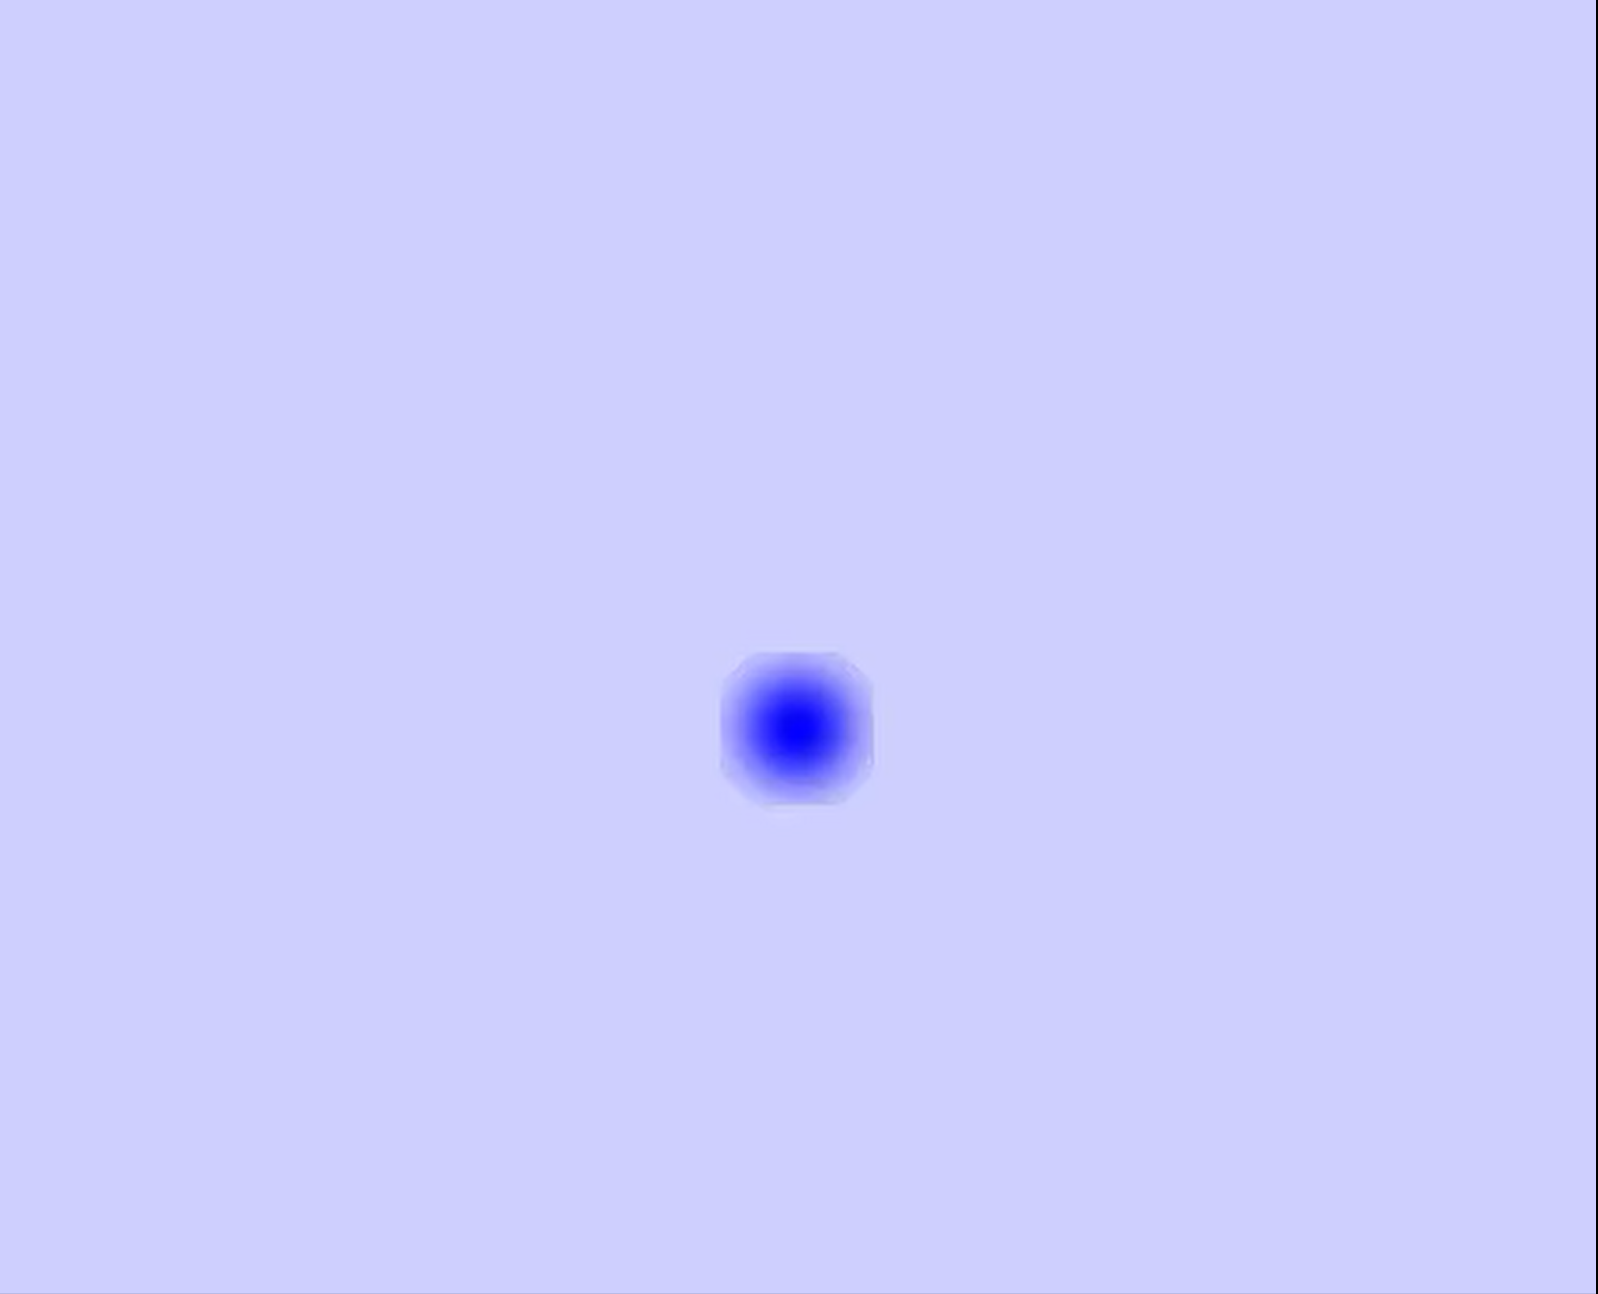
\includegraphics[width=\linewidth]{ph1.png}
        \caption{$t = 0$}
    \end{subfigure}\hfill
    \begin{subfigure}{0.32\linewidth}
        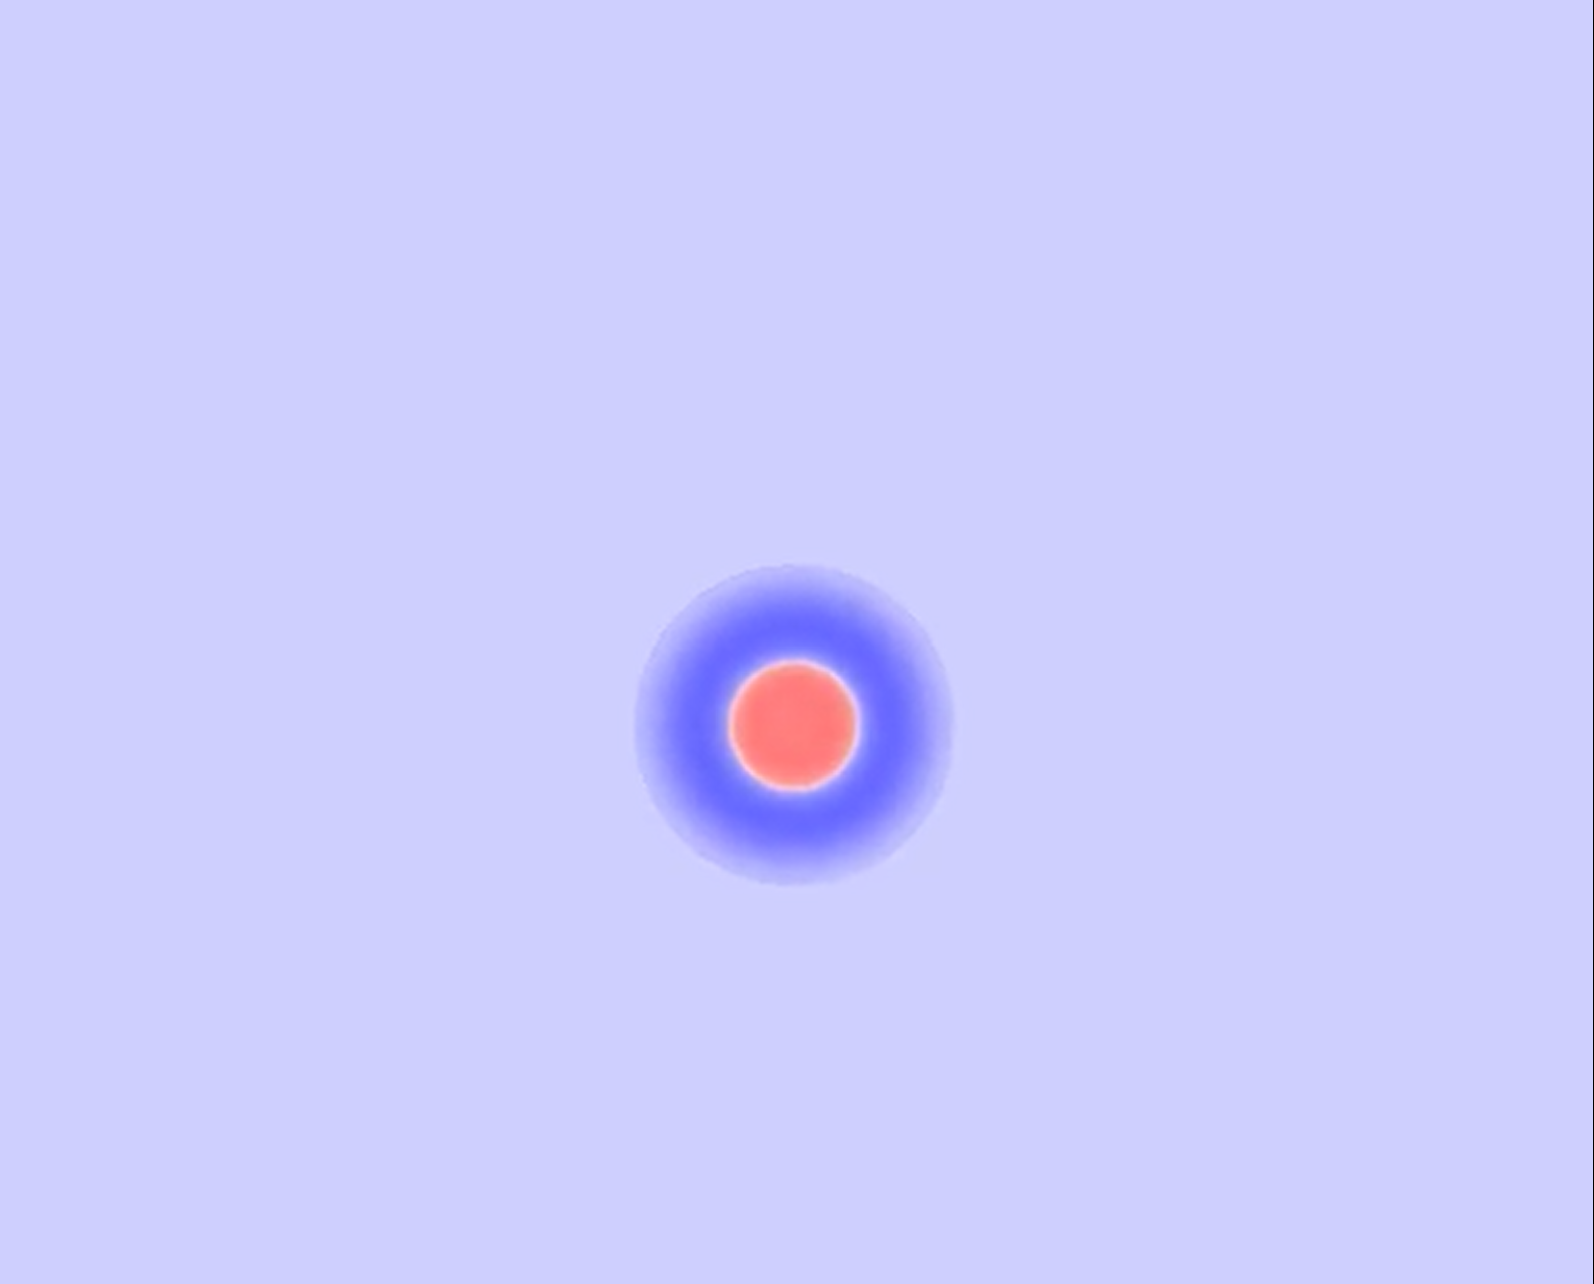
\includegraphics[width=\linewidth]{ph2.png}
        \caption{$t > 0$}
    \end{subfigure}\hfill
    \begin{subfigure}{0.32\linewidth}
        
\includegraphics[width=\linewidth]{ph3.png}
        \caption{$t > N/2$}
    \end{subfigure}
    \caption{Example frames of the colorized wave simulation at different time
    steps. Troughs are rendered in blue, crests in red, and calm regions in
    white; the progressive fading of the colors reflects the damping of the wave
    amplitude.}
    \label{fig:cuda-frames}
\end{figure}

\subsubsection{How the Timings Were Measured}

As explained in Section~\ref{sec:cuda-why}, each frame goes through three GPU
stages: the H2D copy of the grayscale matrix, the kernel that colors it, and the
D2H copy of the RGB result. We measure these three stages separately using CUDA
\emph{events}, which record time on the GPU itself;

Two precautions make the numbers meaningful. First, a \emph{warm-up}: the very
first kernel launch of a program also pays a one-time cost for setting up the
CUDA context and loading the code onto the GPU. If this is charged to the first
measured frame it completely distorts the average, we observed an apparent
$1.22$~ms per frame over $30$ frames versus $0.0096$~ms per frame over $200$, for
the same kernel. We therefore run one untimed ``warm-up'' launch before starting
the measurements, so the reported figures reflect the true steady-state cost.
Second, the writing of the PPM file is disk I/O, not GPU work, so it is
deliberately kept out of the GPU timings; it nevertheless remains the single most
expensive stage of the whole program.

\subsubsection{The Kernel Is Cheap; the Transfers Are Not}

With this methodology the kernel itself turns out to be extremely fast. At
$M=512$ it colors more than $260\,000$ pixels in about $0.01$~ms, and even at
$M=2048$ (over four million pixels) it stays around $0.06$~ms per frame. The
consequence is striking: on the GPU side, the runtime is almost entirely spent on
the two data transfers across the PCIe bus, which together account for roughly
$85$--$90\%$ of the device-side time, while the actual computation is a few
percent.

So, for this problem the arithmetic is cheap and the real cost lies in moving data, here across the PCIe bus between CPU and GPU and, in absolute terms even more, in writing the frames to disk. Recognizing these transfers as the bottleneck is what motivates the optimization in the next subsection.

\subsubsection{An Optimization Beyond the Requirements: Pinned Host Memory}
\label{sec:cuda-pinned}

Optimizing the transfers is not part of the assignment, but since they dominate
the GPU time we investigated the standard technique for this situation:
\emph{pinned} host memory. Ordinary host buffers, allocated with \texttt{malloc},
are \emph{pageable}, meaning the operating system is free to move those memory
pages around (or swap them to disk). Because the GPU's DMA engine copies from
fixed physical addresses, it cannot read pageable memory directly: the driver
must first copy the data into a temporary locked buffer and only then transfer
it, so every byte is copied twice. Allocating the buffers with
\texttt{cudaHostAlloc} instead makes them \emph{pinned} (page-locked): the memory
is nailed to a fixed physical location, the DMA engine reads it directly, and the
intermediate copy disappears.

This comparison is a controlled experiment. Both executables are built from
exactly the same source files; the only difference is a single compile flag
(\texttt{-DUSE\_PINNED\_MEMORY}) that switches the allocation from \texttt{malloc}
to \texttt{cudaHostAlloc}. Any measured difference can therefore be attributed to
the memory type alone, and not to some other change in the code.

Figure~\ref{fig:cuda-pinned} and Table~\ref{tab:cuda-pinned} report a sweep over
the grid size $M$, with each configuration run three times and the median kept
(the node is shared, so repeating guards against the occasional interference from
other jobs). Three things stand out. The transfers become faster, with a peak
speedup of $2.15\times$ at $M=512$. The effective host-to-device bandwidth nearly
doubles, from about $14$~GB/s with pageable memory to about $25$~GB/s with pinned
memory at the larger sizes, the latter close to the practical limit of the PCIe
link. And, as a sanity check, the kernel time is essentially identical in the two
builds ($0.0085$ vs.\ $0.0082$~ms at $M=512$), confirming that pinned memory
affects only the data transfers and not the computation, exactly as expected.

% --------- FIGURA GRAFICI PINNED: scommenta, l'immagine ce l'hai gia' ---------
 \begin{figure}[t]
     \centering
     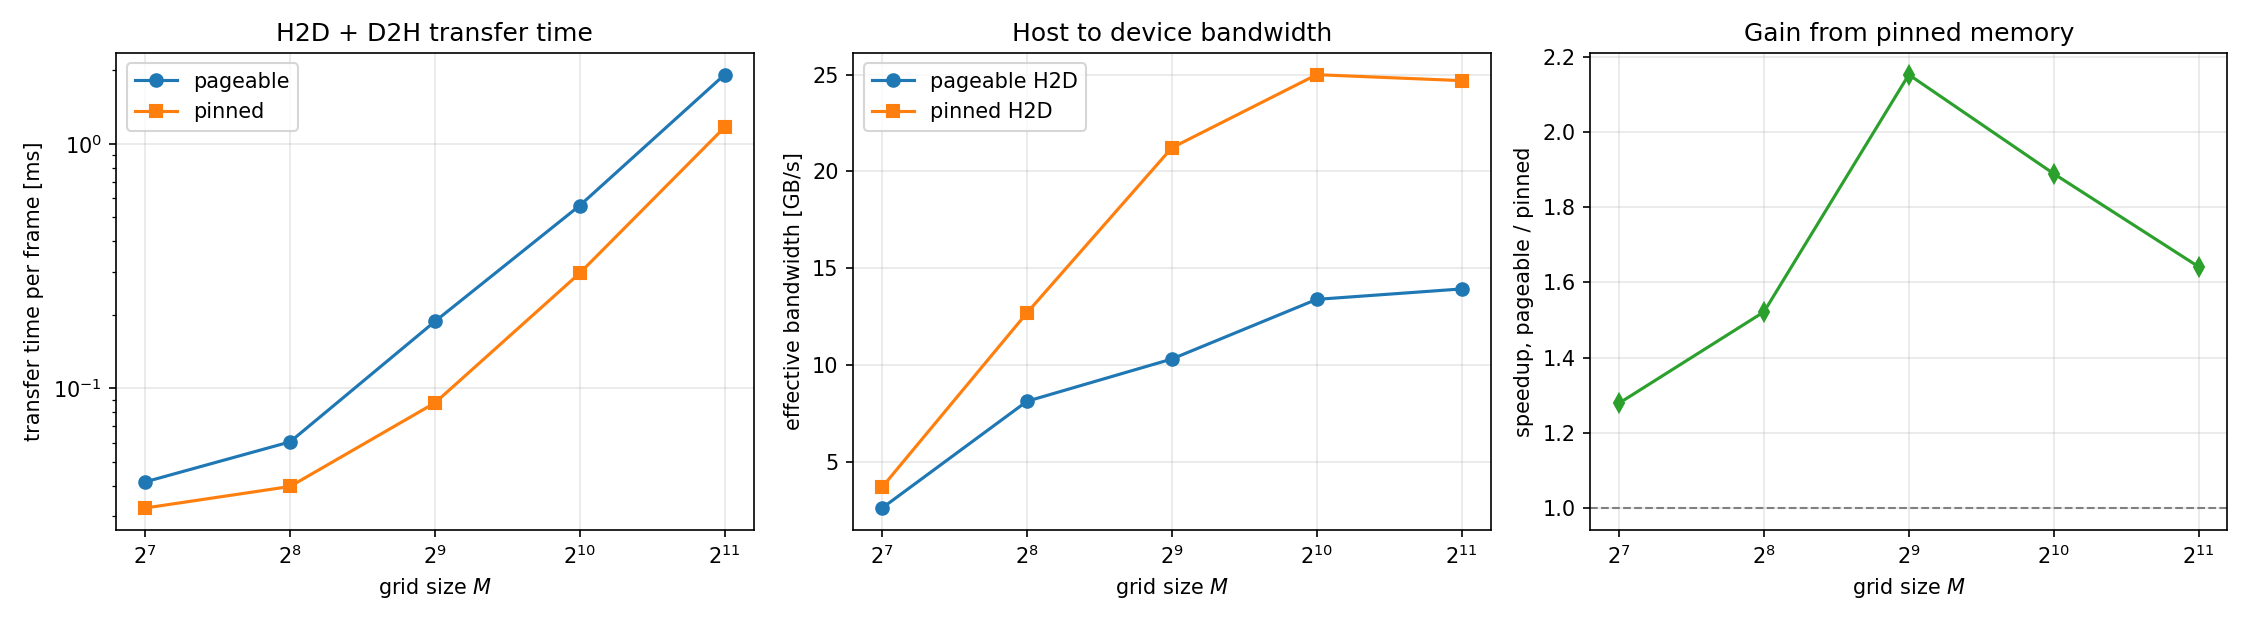
\includegraphics[width=\linewidth]{cuda_pinned_comparison.png}
     \caption{Pageable vs.\ pinned host memory as a function of the grid size $M$.
     Left: combined H2D$+$D2H transfer time per frame. Center: effective
     host-to-device bandwidth. Right: transfer-time speedup of pinned over
     pageable. Medians over three repetitions.}
     \label{fig:cuda-pinned}
 \end{figure}

The speedup is not constant across sizes: it rises up to $M=512$ and then eases
back to $1.6$--$1.9\times$ at the largest grids. The reason is intuitive. At
small sizes the transfer is dominated by a fixed per-call overhead that pinning
does not remove, so the benefit is modest. At intermediate sizes the raw
bandwidth becomes the limiting factor and pinning helps the most. At the largest
sizes the pinned bandwidth saturates near the PCIe ceiling while the pageable
path still gains a little from internal buffering, so the ratio settles. There is
thus a ``sweet spot'' around $M=512$ where pinned memory is most effective.
\begin{table}[t]
    \centering
    \caption{Transfer time per frame (H2D$+$D2H) and effective host-to-device
    bandwidth, pageable vs.\ pinned host memory. Medians over three repetitions.}
    \label{tab:cuda-pinned}
    \setlength{\tabcolsep}{4pt}
    \small
    \begin{tabular}{rrrrr}
        \toprule
        $M$ & pag.\ [ms] & pin.\ [ms] & speedup & BW pin.\ [GB/s] \\
        \midrule
        128  & 0.0412 & 0.0336 & $1.23\times$ & 3.72 \\
        256  & 0.0605 & 0.0398 & $1.52\times$ & 12.71 \\
        512  & 0.1878 & 0.0873 & $2.15\times$ & 21.22 \\
        1024 & 0.5511 & 0.2961 & $1.86\times$ & 24.99 \\
        2048 & 1.9168 & 1.1678 & $1.64\times$ & 24.68 \\
        \bottomrule
    \end{tabular}
\end{table}